\documentclass[12pt,a4paper]{article}
\usepackage[T1]{fontenc}
\usepackage{lmodern}
\renewcommand{\familydefault}{\sfdefault}
\usepackage[brazil]{babel}
\usepackage[left=2.5cm,right=1.5cm,top=2cm,bottom=2cm]{geometry}
\usepackage{booktabs}
\usepackage{tabularx}
\usepackage{graphicx}
\usepackage[font=small]{caption}
\usepackage{indentfirst}
\usepackage{url}

\setlength{\parindent}{1.25cm}
\renewcommand{\arraystretch}{1.2}
\sloppy
\setlength{\emergencystretch}{4em}

\begin{document}

% ---------- capa ----------
\begin{titlepage}
\centering
{\bfseries UniSENAI\\Curso Superior de Tecnologia em Análise e Desenvolvimento de Sistemas\par}
\vspace{6cm}
{\bfseries Daniel Tavares dos Anjos\\João Victor Bagatim\par}
\vfill
{\LARGE\bfseries Trabalho Prático 02: Testes em Telemetria de Fórmula 1\par}
\vspace{0.5cm}
{\large Suíte automatizada com PyTest e Coverage\par}
\vfill
14 de setembro de 2026
\end{titlepage}

\section{Introdução}

A função \texttt{calcular\_estrategia\_pit\_stop}, que recebe \texttt{voltas\_totais},
\texttt{temp\_asfalto}, \texttt{porcentagem\_chuva} e \texttt{desgaste\_pneu}, determina o composto
de pneu e a volta de parada de uma equipe de Fórmula 1.
O número de voltas deve estar entre 30 e 80 e a temperatura do asfalto entre 10 e 60 graus, sob pena
de \texttt{ValueError}; o pneu \emph{Wet} é escolhido com chuva maior ou igual a 50\%, o \emph{Soft}
com temperatura inferior a 25 graus e desgaste maior ou igual a 70\%, e o \emph{Hard} com temperatura
maior ou igual a 25 graus ou mais de 30 voltas restantes. Desgaste de 80\% ou mais emite o alerta de
parada obrigatória.

O código corrigido, a suíte de testes e as instruções de execução estão no repositório
\url{https://github.com/danieltanjos/trabalhao-qa-f1.git}.

\section{Testes de caixa preta}

Os cenários da Tabela~\ref{tab:casos} foram derivados apenas da especificação, com ênfase em análise
de valores-limite. Eles resultam em 22 casos executados, pois vários usam
\texttt{@pytest.mark.parametrize}.

\begin{table}[htbp]
\centering
\caption{Casos de teste funcionais.}
\label{tab:casos}
\small
\begin{tabularx}{\textwidth}{>{\bfseries}clXl}
\toprule
N & Cenário & Entrada (voltas, temp., chuva, desgaste) & Esperado\\
\midrule
1  & Voltas fora do limite      & 29, 81, 0 e $-1$ voltas       & ValueError \\
2  & Temperatura fora do limite & temperatura 9 e 61            & ValueError \\
3  & Valores-limite válidos     & voltas 30 e 80; temp. 10 e 60 & sem exceção \\
4  & Chuva $\geq$ 50\%          & 50, (10, 24, 25 e 60), 50, 10 & Wet \\
5  & Pista fria, desgaste alto  & 50, 24, 49, 70                & Soft \\
6  & Uma só condição de Soft    & (24, 69) e (25, 70)           & diferente de Soft \\
7  & Temperatura elevada        & 50, 25, 0, 10                 & Hard \\
8  & Mais de 30 voltas          & 31, 24, 0, 10                 & Hard \\
9  & Nenhuma regra se aplica    & 30, 24, 0, 10                 & Medium \\
10 & Desgaste de 80\%           & 50, 30, 0, 80                 & alerta; volta 1 \\
11 & Desgaste de 79\%           & 50, 30, 0, 79                 & sem alerta \\
\bottomrule
\end{tabularx}
\end{table}

\section{Cobertura de código}

A verificação estrutural foi executada com \texttt{pytest -{}-cov=estrategia\_f1 -{}-cov-branch
-{}-cov-report=term-missing}. A Figura~\ref{fig:cov} mostra os 22 testes aprovados e as colunas
\texttt{Miss} e \texttt{BrPart} iguais a zero, o que comprova 100\% de cobertura de instruções e de
ramos.

\begin{figure}[htbp]
\centering
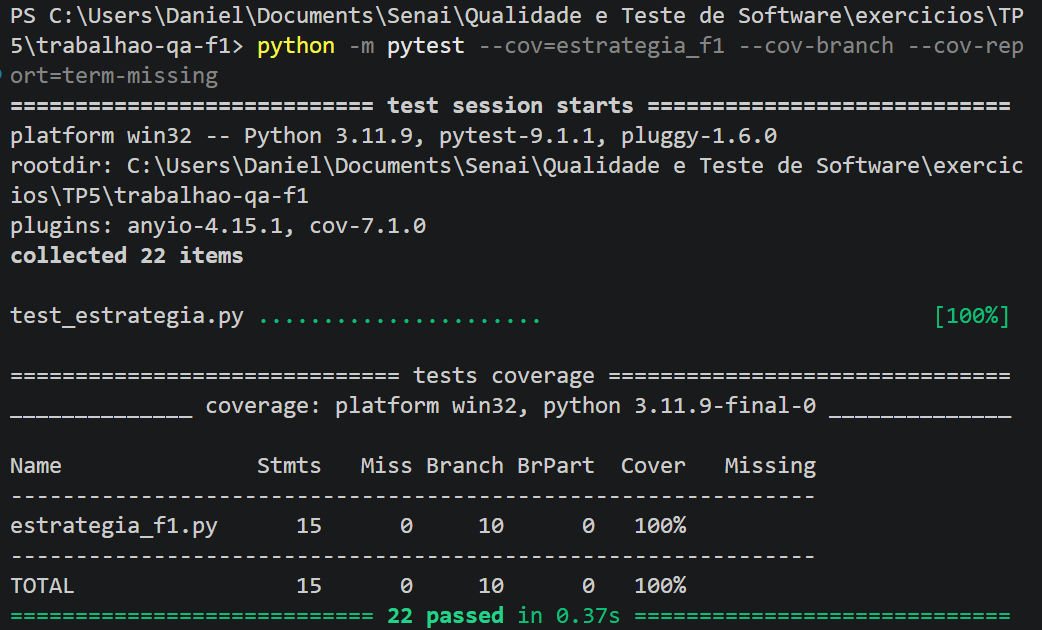
\includegraphics[width=\textwidth]{image.png}
\caption{Saída do terminal com 100\% de cobertura de instruções e de ramos.}
\label{fig:cov}
\end{figure}

\section{Bugs identificados no código base}

Contra o código base original, 10 testes falharam e 12 passaram. A Tabela~\ref{tab:bugs} resume os
três defeitos; após as correções, os 22 testes passam.

\begin{table}[htbp]
\centering
\caption{Defeitos encontrados e respectivas correções.}
\label{tab:bugs}
\small
\begin{tabularx}{\textwidth}{>{\bfseries}clllX}
\toprule
N & Local & Original & Correção & Efeito\\
\midrule
1 & Validação de voltas & \texttt{30 <} & \texttt{30 <=} & Corrida de exatamente 30 voltas rejeitada. \\
2 & Pneu Wet & \texttt{chuva > 50} & \texttt{chuva >= 50} & Chuva de exatamente 50\% não usa pneu de chuva. \\
3 & Pneu Soft & \texttt{or} & \texttt{and} & Uma só condição já seleciona Soft, inclusive onde se exige Hard. \\
\bottomrule
\end{tabularx}
\end{table}

\end{document}
